\section{Grundlagen und Begriffserklärungen}

\subsection{Composable-Enterprise-Architektur}

\subsubsection{Begriffserklärung und Abgrenzung}

\subsubsection{Technologische Konzepte des Composable-Enterprises}

\newpage
\subsection{Integrations- und Bereitstellungsautomatisierung \\von Software}


\subsubsection{Agile und DevOps als Anwendungsentwicklungskonzepte}

Das Hauptaugenmerk eines Composable-Enterprises besteht darin Resilienz und \\Flexibilität aufrecht zu erhalten. Damit soll sichergestellt werden, dass IT-Leistungen in einem sich stetig ändernden Umfeld schnell und risikoarm bereitgestellt werden können. Das traditionelle Wasserfallmodell, welches eine sequenzielle Abfolge der Projektelemente \textit{Anforderung}, \textit{Design}, \textit{Implementierung}, \textit{Test} und \textit{Betrieb} vorgibt, besitzt dabei signifikante Limitationen. Die in dieser Methodik detailliert durchgeführte Vorabplanung, kann in der Realität aufgrund unvorhersehbarer Externalitäten selten eingehalten werden. Auch die starre Abfolge der Projektphasen mindert besonders zu fortgeschrittenen Zeitpunkten des Vorhabens den Spielraum für Anpassungsmöglichkeiten \cite{Vivenzio.2013}[5]. Dies resultiert nicht nur ein einem Anstieg der Kosten sondern führt ebenfalls dazu, dass IT-Projekte länger als geplant ausfallen \cite{Vieweg.2015}[41]. Als Reaktion haben sich agile Vorgehensmodelle zunehmend innerhalb der Projektmanagementlandschaft etabiliert.
Im Gegensatz zum Wasserfallmodell, welches eine umfassende Vorab-Planung vorsieht, wird das Vorhaben in einer agilen Entwicklung in viele Teilprojekte, sog. \textit{Sprints}, segmentiert (s. Abb. \ref*{fig:Agile_Cycle}) \cite{Goll.2015}[87]. 
\begin{center}
	\begin{figure}[H]
		\centering
		\scalebox{0.5}{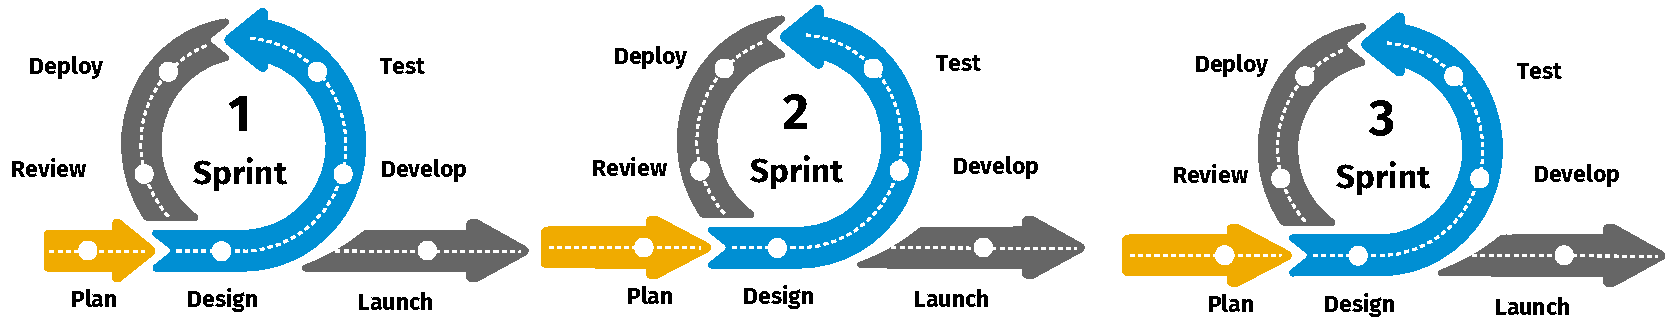
\includegraphics{Agile_Cycle}}
		\caption[Exemplarische Abfolge eines agilen Entwicklungszykluses]{Exemplarische Abfolge eines agilen Entwicklungszykluses. In Anlehnung an K\&C \cite{KUC.2021}.}
		\label{fig:Agile_Cycle}
	\end{figure}	
\end{center}
\vspace*{-15mm} Sprints sind Durchläufe, welche i.d.R. einen Zeitraum von ein bis vier Wochen umfassen, in welcher die Fertigstellung einer vor dem Teilprojekt definierten Aufgabenkontingente vorgesehen ist. Am Ende jeden Sprints soll dabei ein potenziell an den Kunden auslieferbares Produkt entstehen. Dies erlaubt eine schnelle Bereitstlellung funktionsfähiger Software, was neben der Erhöhung der Kundenzufriedenheit ebenfalls in einer Optimierung der Planungsgenauigkeit resultiert. So kann das nach Ablauf des Sprints potenziell an die Stakeholder auslieferbare Artifakt als Feedback-Grundlage für weitere Anpasssungen verwendet werden \cite{K&C.2021}[39]. 
Die dabei bereitgestellten Features können vom Kunden im Regelbetrieb geprüft und auf Anforderungserfüllung untersucht werden \cite{Gloger.2016b}[180]. Damit kann auf während des Reviews festgestellte Mängel im unmittelbaren Folge-Sprint reagiert werden. Dieser Sprint-Review-Zyklus wird solange durchgeführt, bis alle Kundenbedürfnisse erfüllt sind und das Vorhaben als abgeschlossen gilt.
Inneralb der letzten Dekade haben sich dabei diverse auf agilen Prinzipien basierenden Vorgehensmodelle, wie Scrum, Kanban oder \ac*{XP} in der Softwareentwicklung etabliert. Obwohl einige dieser Methoden zur erfolgreichen Zusammenarbeit innerhalb der Entwicklungsteams beigetragen haben, bleibt das sog. Problem der \textit{Letzten Meile} bestehen \cite{Qentelli.20230305}. Traditionell erfolgt eine funktionale Trennung der Entwickler- und IT-Betriebler-Teams. Das Problem der Letzten Meile beschreibt dabei, dass aufgrund ausbleibender Kooperation der Entwicklungs- und Betriebsteams der Programmcode nicht auf die Produktivumgebung abgestimmt ist. Die Verzögerung der Markteinführungszeit resultiert damit in einem geminderten Wertschöpfungsprozess und somit einer Abnahme des Ertragspotenzials bzw. in einer Erhöhung der Betriebskosten \cite{Halstenberg.2020}[1]. Und scheint dieses Phänomen kein Einzelfall zu sein. So geht aus der von McKinsey veröffentlichen Studie \textit{The Business Value of Design 2019} hervor, dass durchschnittlich 80 Prozent des Unternehmens-IT-Budgets zur Aufrechterhaltung des Status Quo verwendet wird. Stattdessen fodert das Beratungshaus eine Rationalisierung der Bereitstellung und des Betriebs von Software, um finanzielle Mittel für wertschöpfende Investitionen zu maximieren \cite{.20230305}. Abhilfe schaffen kann dabei das in der Literatur als \textbf{\ac*{DevOps}} bekannte Aufbrechen organisatorischer Silos zwischen Entwicklung und dem IT-Betrieb \cite{Halstenberg.2020}[1]. 
Dabei stellt DevOps keine neue Erfindung dar. Stattedessen werden einzelne bereits bewährte Konzepte, wie die agile Softwareentwicklung, zu einem umfassenden Rahmenwerk konsolidiert. Prägnant zusammenfassen lässt sich das DevOps-Konzept durch das Akronym CAMS: \textit{Culture (Kultur)}, \textit{Automation (Automatisierung)}, \textit{Measurement (Messung)} und \textit{Sharing (Teilen)} \cite{Halstenberg.2020}[5]. Dabei gilt \textit{Kultur} als das wohl wesentlichste DevOps-Erfolgselement. Diese Norm bezweckt eine Zusammenarbeitskultur, welche sich über alle Ebenen eines Unternehemens erstreckt. Operative Entscheidungen sollen dabei auf die Fachebenen herunterdelegiert werden, welche aufgrund ihrer spezifischen Expertise am geeignesten sind, diese Dispositionen zu verabschieden \cite{Halstenberg.2020}[5]. Eine \textit{Automatisierung} von bei der Softwarebereitstellung anfallenden Prozessen, ermöglicht sich wiederholende manuelle Arbeit zu elemenieren. Eine hochautomatisierte Infrastrukur kann ebenfalls zur Ratsionalisierung und damit zur Senkung der IT-Betriebskosten beitragen. Der dabei erzielte Einfluss wird anhand verschiedener DevOps-Kennzahlen bemessen (\textit{Messung}). Neben der Systemverfügbarkeit und der Instandsetzungszeit ist insbesondere der \textit{Time-to-Market} eine signifikante Metrik \cite{Halstenberg.2020}[7]. 

\begin{center}
	\begin{figure}[H]
		\centering
		\scalebox{0.38}{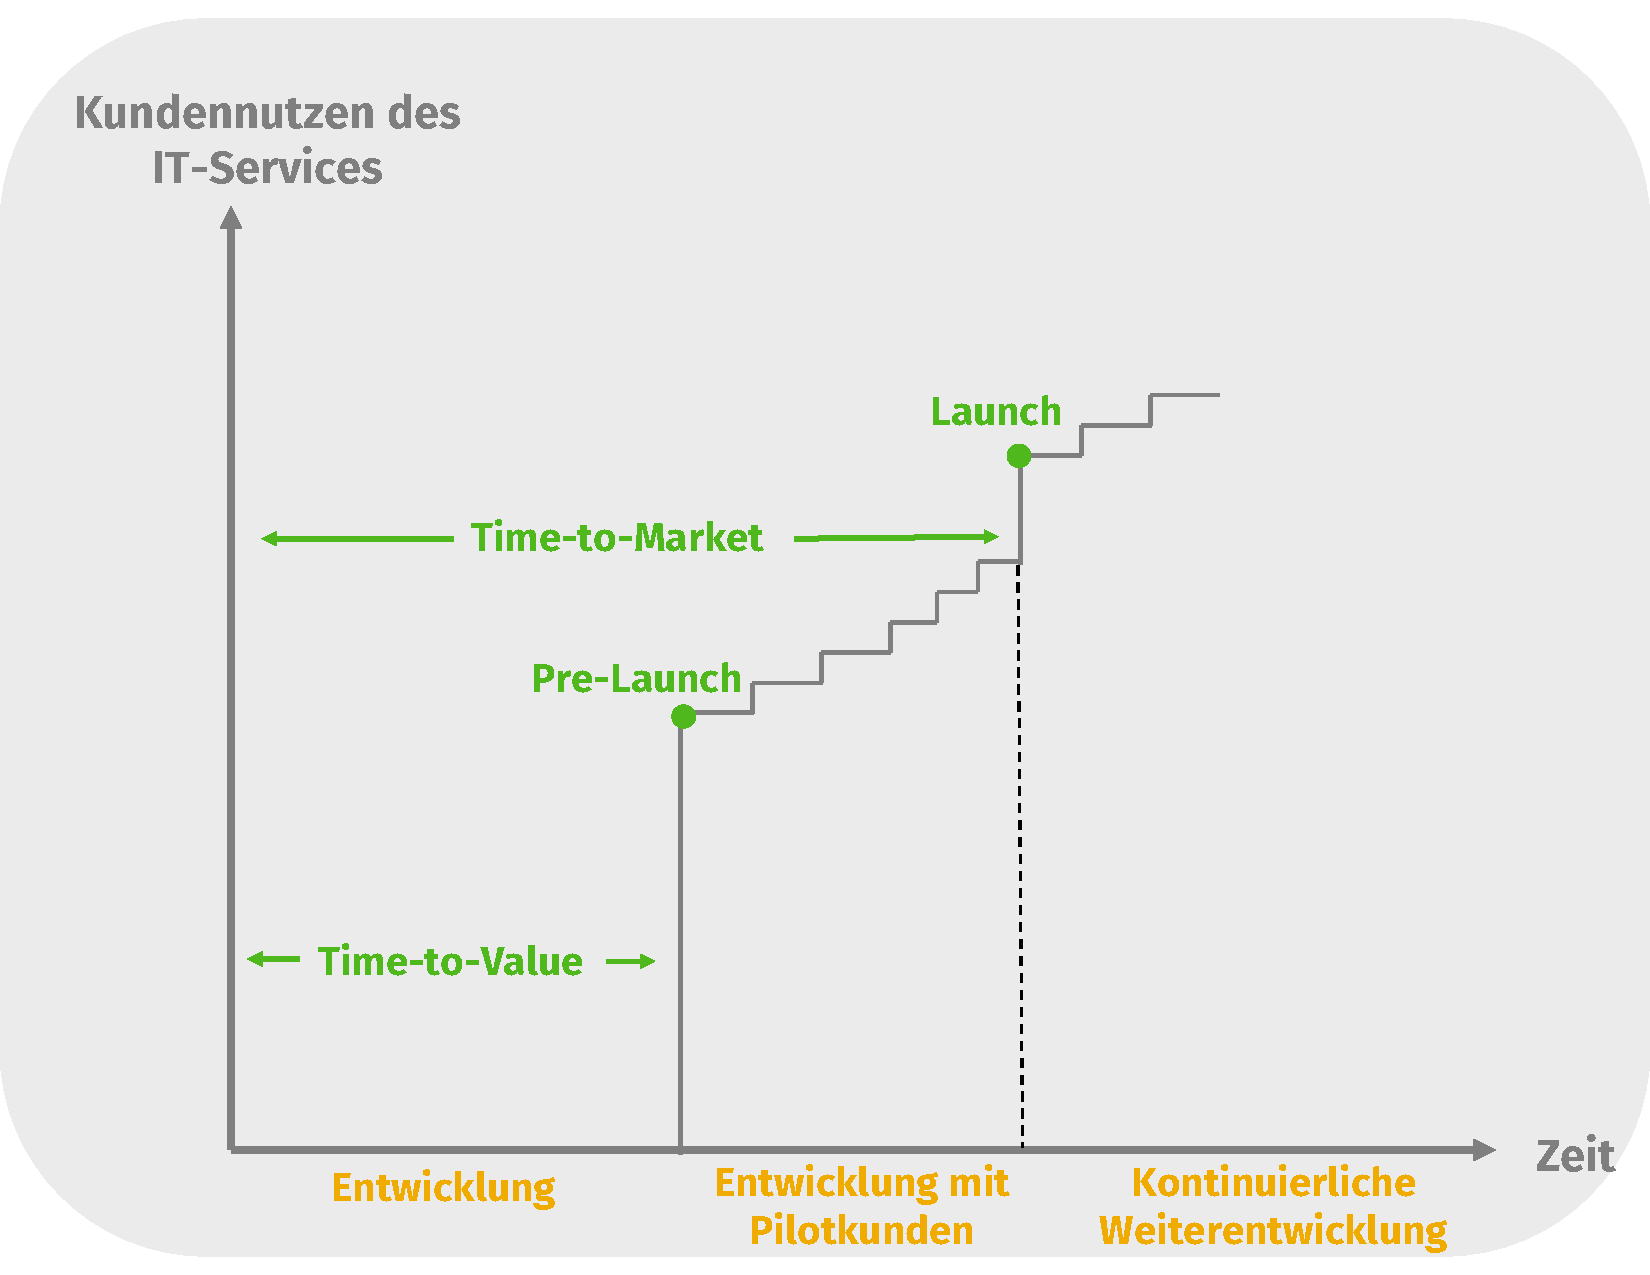
\includegraphics{TTM}}
		\caption[Zeitliche Darstellung des Kundennutzen von IT-Services]{Zeitliche Darstellung des Kundennutzen von IT-Services. In Anlehnung an Halstenberg \cite{Halstenberg.2020}[9].}
		\label{fig:TTM}
	\end{figure}
\end{center}
\vspace*{-10mm}
Der Time-To-Market beschreibt die Zeitspanne zwischen Entwicklungsentstehungsprozess und der Markteinführung der IT-Services \cite{Vesey.1992}[141]. Auch der \textit{Time-to-Value} erhält zunehmend eine erhöhte Aufmerksamkeit. Im Gegensatz zum Time-to-Market wird hier nicht die Zeit bis zur Komplett-Einführung, sondern bis zum ersten Kundennutzen bemessen. Obwohl der im Time-to-Value bereitgestellte IT-Service mölglicherweise Verbesserungspotenzial bietet, überwiegt der mit der initialen Auslieferung herbeigeführte Mehrwert. Dabei ermöglicht eine solche Früheinführung einen Vorpsrung gegenüber anderen Konkurrenten. So ist es dem Softwareunternehmen bereits gelungen erste Kunden zu finden, deren Input und Feedback möglichst rasch erfasst und verarbeitet werden kann \cite{Halstenberg.2020}[9]. Softwareunternehmen können IT-Services ab dem Pre-Launch somit sukkzessive und ressourcenoptimiert unter Zusammenarbeit mit den Pilotkunden erweitern. Auch Adam Caplan leitender Strategieberater bei Salesforce empfiehlt angesichts der bei der Integration der IT-Systemen entstehenden Komplexität, Software schnellstmöglichst in Produktivumgebung zu testen \cite{Vesey.1992}. Aus diesen Erfahrungen sollen dann Best Practises entwickelt werden, welche dann innerhalb von Teams und organisationsübergreifend weitergegeben werden sollten (\textit{Teilen}) \cite{Halstenberg.2020}[7]. 

\subsubsection{CI/CD-Pipelines zur Softwarebereitstellung}

DevOps beschreibt eine Philosophie, mit welcher die Zusammenarbeit zwischen Entwicklungs- und Betriebsteams gefördert werden soll. Ein integraler Bestandteil des DevOps-Rahmenwerks ist neben verschiedener agiler Entwicklungsmethoden ebenfalls \ac*{CI/CD}. CI/CD ist eine Softwareentwicklungsmethode, welche zur Verbesserung der Qualität bzw. zur Senkung der Entwicklungszeit von IT-Services beitragen soll. Abhilfe schaffen soll dabei eine Pipeline, welche alle Schritte von Codeintegration bis Bereitstellung der Software automatisiert. Hauptaugenmerk liegt dabei darauf, Software zuverlässiger und häufiger bereitzustellen. Alle in diesem Prozess anfallenden Aktivitäten sind dabei dem CI/CD-Cycle zu entnehmen (s. Abb. \ref*{fig:CICD_Cycle}).
\begin{center}
	\begin{figure}[H]
		\centering
		\scalebox{0.5}{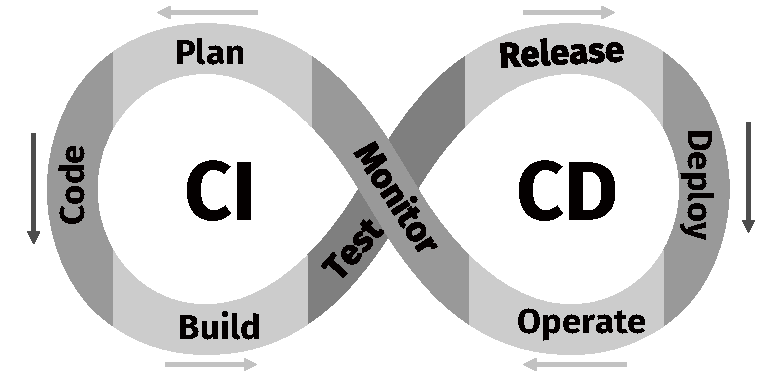
\includegraphics{CICD_Cycle}}
		\caption[Aktivitäten im CI/CD-Prozess]{Aktivitäten im CI/CD-Prozess. In Anlehnung an.}
		\label{fig:CICD_Cycle}
	\end{figure}
\end{center}
\vspace*{-10mm}
Der \acs*{CI}-Prozess (Continuous-Integration-Prozess) bezweckt, dass lokale Quellcode\-änderungen in kurzen Intervallen und so schnell wie möglich in eine zentrale Codebasis geladen werden. Das frühzeitige Integrieren von Code soll dabei zu einer unmittelbaren und zuverlässigen Fehlererkennung innerhalb des Entwicklungsvorhabens beitragen. Der erste Schritt im CI-Prozess umfasst die \textit{Planung} zu entwickelnder Services (s. Abb. \ref*{fig:CICD_Cycle}). Dabei soll festgestellt werden, welche Anforderungen eine Lösung besitzt bzw. welche Softwarearchitekturen sowie Sicherheitsmaßnahmen implementiert werden sollten. Im Sinne der agilen Entiwcklung wird dabei das aus dem \textit{Monitoring} erhobene Feedback berücksichtig und angewendet. Um sicherzustellen, dass die in der Planung entworfene Anwendungsarchitektur auf das Design des Produktivsystems abgestimmt ist, sollte zu jedem Zeitpunkt das Know-How der Betriebsteams einbezogen werden. Nach erfolgreichem Entwurf zu implementierender Anwendungsfeatures beginnt die Entwicklung der IT-Services (\textit{Code}: s. Abb. \ref*{fig:CICD_Cycle}). Arbeiten hierbei mehrere Entwickler parallel an dem selben IT-Service, wird der entsprechende Quellcode in sog. Repositories wie Github oder Bitbucket ausgelagert. Ein Repository stellt dabei einen zentralen Speicherort dar, welcher das Verfolgen sowie Überprüfen von Änderungen und ein paralleles bzw. konkurrierendes Arbeiten an einer gemeinsamen Codebasis ermöglichen soll. Der in dem Repository archivierte Hauptzweig (Master-Branch) stellt dabei eine akutelle und funktionsfähige Version des Codes dar. Dieser mit verschiedenen Validierungsprozessen überprüfte Code, kann dabei zu jeder Zeit in der Produktionsumgebung bereitgestellt werden. (s. Abb. \ref*{fig:VCS}). Im Sinne der agilen Entwicklung werden dabei große Softwareanforderungen, sog. Epics, in kleine Features segmentiert, welche in separate Feature-Branches ausgelagert werden. Diese sind unabhängige Kopien des Hauptzweiges, in welcher ein Entwickler Änderungen vornehmen können ohne Konflikte in der gemeinsamen Codebasis zu verursachen.
\begin{center}
	\begin{figure}[H]
		\centering
		\scalebox{0.8}{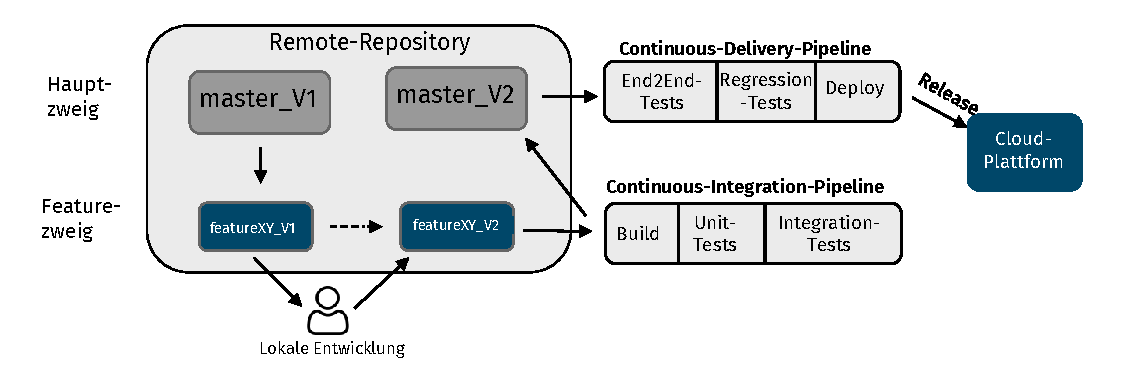
\includegraphics{VCS}}
		\caption[Versionskontrollsysteme zur Verwaltung von Quellcode]{Versionskontrollsysteme zur Verwaltung von Quellcode. In Anlehnung an.}
		\label{fig:VCS}
	\end{figure}
\end{center}
\vspace*{-10mm}
Nach Fertigstellung der Funktionalitäten sollte der um die Features erweiterte Quellcode so schwird sichergestellt, dass der Code stets stabil, also funktionsfähig ist und keine Konflikte mit dem akutellen Code des Hauptzweiges aufweist. Dabei wird eine Validierung des Code anhand der \ac*{DoD} fociert. Die DoD ist eine in der Planungsphase festgelegte Anforderungsspezifikation, welche zur  Integration in den Master-Branch erfüllt werden muss. Im Rahmen dieser Norm sind Entwickler dazu angehalten für jedes implementierte Feature einen der DoD entsprechenden Test zu entwerfen. Anschließend wird die Applikationen zu einem ausführbaren Programm kompiliert (\textit{Build}) anhand welcher verschiedeneste Tests ausgeführt werden. Dafür können je nach Programmiersprache verschiedene Build-Tools, wie Maven für Java oder NPM für Javascript verwendet werden. Die dabei durchgeführten Überprüfungen, auch \enquote*{Smoke-Tests}, sollen  sicherstellen, dass zu jeder Zeit in rudementärgetesteter Code bereit steht und grundlegende Funktionalitäten sowie Schnittstellen erwartungsgemäß operieren. Der in den Entwicklungszweig bereitgestellte Code wird dabei überwiegend anhand schnell durchführbarer Tests überprüft. Die Durchführung von ressourcenschonenden Tests hat dabei insbesondere zwei Ursachen. Der Hauptaugenmerk von Continuous Integration liegt insbesondere darauf, dass der lokale Entwicklungscode so oft wie möglich in das gemeinsame Repository geladen wird. Aufwendige Tests mit einer langen Laufzeit würden Entwickler somit hemmen Code in einer hohen Frequenz bereitzustellen. Statt den gesamten Code vor einem Release vor zusammenzuführen (Merge Day), soll sichergestellt werden, dass Fehler und Konflikte so schnell wie möglich entdeckt und behoben werden. Dabei durchgeführte Tests sind i.d.R. Unit- und sowie Integrationtests.
\begin{center}
	\begin{figure}[H]
		\centering
		\scalebox{0.3}{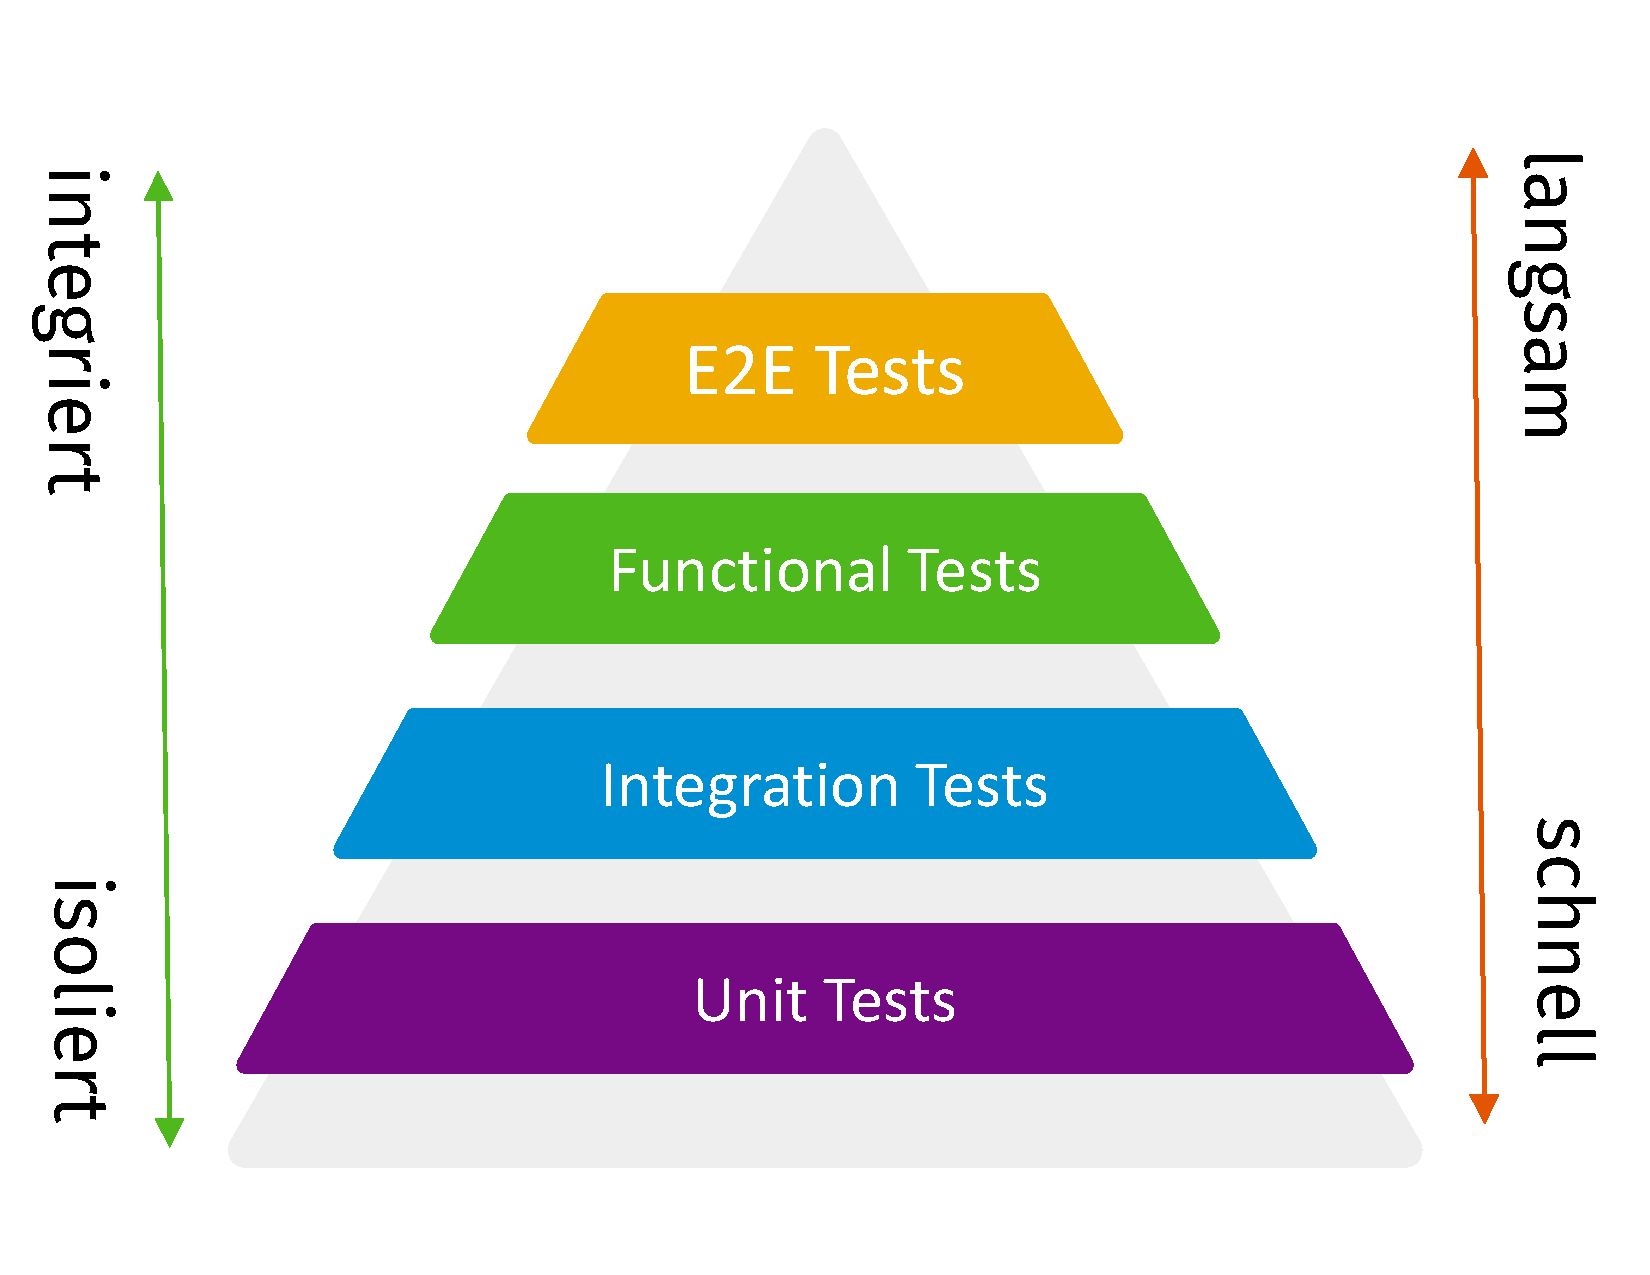
\includegraphics{Tests}}
		\caption[Hierarschische Darstellung von Softwaretests]{Hierarschische Darstellung von Softwaretests. In Anlehnung an.}
		\label{fig:Tests}
	\end{figure}
\end{center}
\vspace*{-10mm}
Unit Tests befinden sich dabei auf unterster Hierarchieebene der Test-Pyramiede (s. Abb. \ref*{fig:Tests}). Mit Unit Tests wird die Funktionale Korrektheit kleinster Einheit überprüft. Dies können etwa unabhängige Komponenten wie einzelne Methoden einer Klasse sein. Der Zweck der Unit-Tests besteht dabei in einer von externen Einflüssen und Daten unabhängien Überprüfung der einzelnen Komponenten. Um bei der Bereitstellung neuer Funktionalitäten ebenfalls das Zusammenspiel einzelner Komponenten zu überprüfensdasd werden Integration Tests durchgeführt. I.d.R. werden diese in einer White-Boxed-Umgebung abgewickelt. Dies impliziert, dass der Entiwckler des Integration-Tests Kenntnis von dem Quellcode, den verwendeten Technologien sowie der Awendungsarchitektur besitzten. Bei einem solchen Tests, können also gezielt Aspekte, wie der Austausch eines Nachrichtenmodells bei der Kommunikation zweier Web-Services untersucht werden. Nachdem einzelne Funktionalitäten entwickelt und erfolgreich gestet werden, werden diese zu den Änderungen im Hauptzweig zusammengeführt. Ab diesem Zeitpunkt beginnt das Continous Delivery.  Während Continuous Integration insbesondere den Prozess der kontinuierlichen Integration von Quellcode in ein gemeinsames Repository bezweckt, wird mit Continuous Delivery die Automatisierung der Anwendungsbereitstellung gesteuert. Applikationen sollen somit ohne große Verzögerungen in die Produktivumgebung und somit zum Kunden ausgelifert werden. In der Theorie sollte der CD-Prozess automatisch und unmittelbar nach Ablauf aller CI-Aktivitäten und somit nach Integration ggdes Codes in den Hauptzweig angestoßen werden. In der Praxis wird hierbei jedoch häufig ein manueller Schritt zwischengestellt, womit sichergestellt werden kann, dass die Anwendung erst in die Produktionsumgebung ausgerollt wird nachdem alle Gesichtspunkte der Bereitstellung überprüft wurden. Zu Beginn des CD-Prozesses wird das in die Produktivumgebung bereitzustellende Artifakt 
über eine Deployment-Pipeline in eine Staging-Area gelanden. Bei der Staging-Area handelt es sich dabei um ein System, welches zwischen der Entwicklugns- und er Produktivumgebung liegt. Dabei werden Konfigurationen des Stating-Systems möglichst produktionsähnlich angelegt. Neben den Datenbanken, werden hierbei auch Serverkonfigurationen, wie Firewall- oder Netzwerkeinstellungen von dem Produktivsystem übernommen. Somit soll sichergestellt werden, dass eine neue Version der Anwendung unter den Bedingunen die der Produktionsumgebung möglichst getestet wird. Wie im CI-Prozess, werden innerhalb dieser Phase Unit- und Integrationtests durchgeführt. Diese sind i.d.R. deutlich rechenintesniver und besitzen eine längere Ausführungszeit. In der Staging Area werden unterdessen auch in der Test-Pyramide (s. Abb. \ref*{fig:Tests}) höher gestufte Tests ausgeführt. Dazu gehören etwa \textit{Functional-Tests}. Mit diesen werden die Planungsphase festgelegten Anforderungen bzw. Funktionen der Anwendung überprüft. So etwa überprüft werden, ob bei der Eingabe einer Benutzer-Passswort-Kennung ein korrekter Authorisierungstoken übergeben wird. Genau wie der Integrationstest, umfasst ein Funct die Überprüfung mehrere Komponenten. Während bei Integrationstests jedoch überprüftion lediglich die generelle Durchführbarkeit einer Operation, wie z.B. ob die Abfrage nach einer Authorisierungstoken überhaupt möglich ist, wird bei einem Functional Test die Korrektheit der spezifischen Ausgabe überprüft. End-to-End-Tests liegen dabei in der Test-Pyramide eine weitere Hierarchieebene höher. Mit diesen soll sichergestellt werden, dass die gesamten Anforderungen der verschiedenen Stakeholder erfüllt werden. Hierbei wird ein vollstädniges Anwenderszenario von Anfang bis Ende getestet. Ein solches Szenario kann im Kontext eines E-Commerce-Webshops etwa das Anmelden mit Benutzername, das Suchen eines Produktes und das anschließende Bestellen umfassen. Zusätzlich zu den hier aufgeführten deduktiven Tests, werden in der Deployment-Pipeline i.d.R. auch Codeanalysen durchgeführt. Hier wird etwa überprüft, welcher prozentaule Anteil des Codes durch Unit-Tests überprüft wird oder Qualitätsstandards, bei welchen auf Schwachstellen verwendeter Code-Patterns bzw. Dublikate überprüft wird. Hat die Version alle Tests erfolgreich durchlaufen wird das überprüfte Artifakt auf die Cloud-Plattform gelanden (\textit{Deploy}). Je nach Bereitstellungsstrategie (s. \ref*{sec:sec:Bereitstellungs_Strategien}), wird die Anwendung dann unmittelbar oder erst nach weiteren Überprüfungen für den Kunden zugänglich gemacht. Um eine ordungsgemäße Ausführung der Anwendung in der Produktionsumgebung sicherzustellen wird die bereitgestellte Awendung im letzten Schritt des CD-Prozesses überwacht (\textit{Monitoring}). Dabei wird das Applikationstracking i.d.R. unabhänig von der CI/CD-Pipeline auf den der Cloud-Platform betrieben. Wichtige Überwachungselemente sind Infrastruktur sowie Anwendungs-Monitoring. Beim Infrastruktur-Monitoring werden Metriken wie CPU-, Speicher- und Netzwerklast der Server, Datenbanken und Netzwerkkomponenten untersucht. Das Anwendungs-Monitoring umfässt dabei die Überwachung der Funktionalitäten sowie der Applikation selbst. Hierbei werden Informationen wie Anfragen pro Sekunden, die Anzahl der Benutzer oder in Log-Dateien gesammelte Fehlercodes analysiert. 

\subsubsection{Strategien zur Bereitstellung von Neuentwicklungen}
\label{sec:Bereitstellungs_Strategien}
Nachdem das Artifakt auf einer virtuellen Maschine einer Cloud-Instanz installiert und ausgeführt wird entscheiden verschiedene Strategien über die Inbetriebnahme der neuen Softwareversion. Mit dieser Strategie wird festgelegt, wie Nutzeranfragen innerhalb des Produktivssystems von der alten auf die neue Version der Anwendung übermittelt wird.
\begin{center}
	\begin{figure}[H]
		\centering
		\scalebox{0.4}{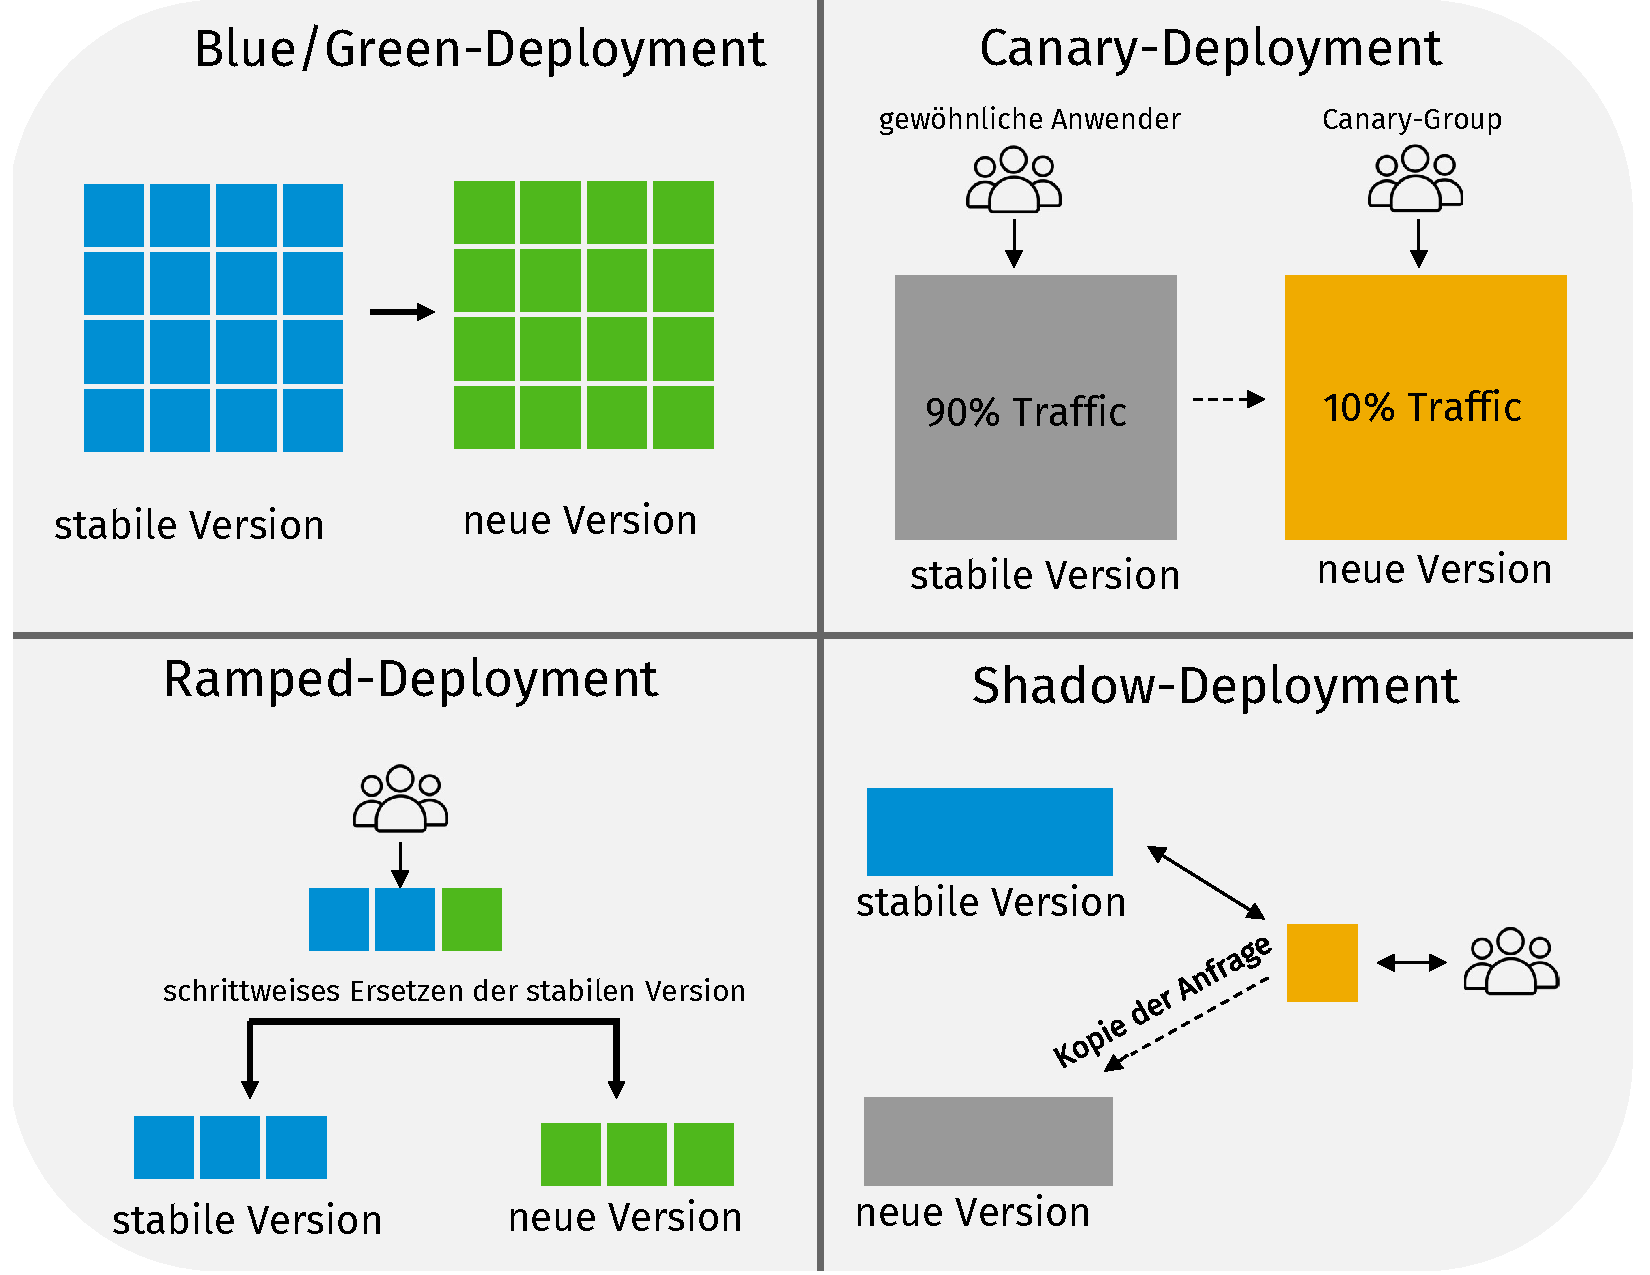
\includegraphics{Deployment_Strategies}}
		\caption[Strategien zur Bereitstellung von Software]{Strategien zur Bereitstellung von Software. In Anlehnung an.}
		\label{fig:DS}
	\end{figure}
\end{center}
\vspace*{-10mm}
Eine häufig verwendete Deployment-Strategie ist dabei das \textit{Blue/Green-Deployment}. Hierbei wird neben der stabilen aktuellen Anwendung (die blaue Version) ebenfalls eine Insanz mit der neuen Anwendung (die grüne Version) betrieben. Die Nutzeranfragen werden dabei von dem Lsatverteilungsservice erst nach Validierung aller Tests umgeschalten. Dazu gehören neben den in der CI/CD-Pipeline definierten Tests ebenfalls Abnahmetest der Qualitätssicherung ausgeführt. Dies sind manuelle Test, in welchen Funktionen, Benutzeroberfläche sowie die Anwenderfreundlichkeit überprüft werden. Statt wie beim Blue/Green-Deployment die neue Version zu einem Zeitpunkt für die gesamte Nutzerbasis bereitzustellen, zielt das \textit{Canary-Deployment} darauf, die Nutzungslast kontinuierlich und sukkzessive auf die neue Anwendung umzuleiten. Hierfür wird die Anwendung vorerst einer kleinen Anzahl an Benutzer bereitgestellt. Eine Canary-Gruppe sollte dabei so zusammengestellt werden, als dass diese die Gesamtzielgruppe möglichst gut represäntiert. Anhand dieser soll dann der fehlerfreie Betrieb der neuen Anwendung überprüft und ggf. Anpassung vorgenommen werden, bevor diese für alle Nutzer freigeschalten wird. Für Anwendungen mit einer hohen Service-Level-Architektur sowie kritischen IT-Systeme wird i.d.R. die \textit{Ramped-Deployment-Strategy} verwendet. Diese ermöglicht eine präzise Kontrolle für horizontalskalierte Services. Bei einer horizontalskalierten IT-Infrastruktur wird die Rechenkapizität einer Anwendung durch das Hinzufügen indentischer Services. Mit dieser Architektur ermöglicht sich eine bessere Lastverteilungen, da Anfragen unabhänig von dem Kontext auf unterschiedliche  Instanzen verteilt werden können. Mit Beginnen des Ramped-Deployment-Prozesses wird die neue Softwareversion schrittweise auf den horizontalen Instanzen ausgerollt. Dabei ist es möglich, dass zu Beginn des Ausrollens die ersten aktualisierten Instanzen lediglich für bestimmte Anwender, sog. Ramped-Gruppen bereitgestellt wird. Dabei ermöglicht es sich für die DevOps-Teams neben der Analyse der Anwendungsmetriken ebenfalls das Feedback der Ramped-Gruppen zu erfassen. Eine aufwendigere jedoch mit weniger Risiko behaftete Bereitstellungsstrategie stellt das \textit{Shadow-Deployment} dar. Dabei wird neben der Instanz der akutellen Version ebenfalls ein sog. Shadow-Model auf der Infrastrukur betrieben. Dieses Shadow-Model beinhaltet dabei die neue Version der Anwednung, kann jedoch nicht unmittelbar von den Nutzer verwendet werden, sondern stellt dem Namen entsprechend eine hinter der stabilen Version gelagerte Instanz dar. Anfragen der Anwender werden von dem Cloud-Service stets auf die aktuelle Version weitergeleitet, verarbeitet und beantwortet. Eine Kopie dieser Anfrage wird dabei jedoch ebenfalls an das Shadow-Model weitergeleitet und zur Laufzeit prozessiert. Die Verwendung des in der Produktionsumgebung abgewickelten Netzwerkverkehs, ernöglicht den Entwickler somit eine anwendungsbezogene Überprüfung entwickelter Features. 